% !TeX spellcheck = fr_FR
\documentclass[a4paper,11pt,oneside,roman]{article}
    \usepackage[utf8]{inputenc}
    \usepackage[T1]{fontenc}
    \usepackage[top=2cm, left=2cm, right=2cm, bottom=2cm]{geometry}
    \usepackage[francais]{babel}
    \usepackage[hidelinks=true]{hyperref}
    \usepackage{listings}
    \usepackage{color}
    \usepackage{amsmath}
    \usepackage{graphicx}
    \usepackage{amssymb}
    \usepackage{natbib}
    \usepackage{float}
    \usepackage{hyperref}
    \usepackage{advdate}
    \usepackage{caption}
    \usepackage{subcaption}
    
    \floatplacement{figure}{H}
    
    \definecolor{dkgreen}{rgb}{0,0.6,0}
    \definecolor{gray}{rgb}{0.5,0.5,0.5}
    \definecolor{mauve}{rgb}{0.58,0,0.82}
    
    \linespread{1.3} %space between lines
    \setlength{\parskip}{1em}  %space between paragraphs
    
    \begin{document}
    
    \begin{titlepage}
    
        \newcommand{\HRule}{\rule{\linewidth}{0.5mm}} % Defines a new command for the horizontal lines, change thickness here
        
        \center % Center everything on the page
         
        %----------------------------------------------------------------------------------------
        %	HEADING SECTIONS
        %----------------------------------------------------------------------------------------
        
        \textsc{\LARGE Université de Technologie de Compiègne}\\[0.5cm] % Name of your university/college
        \textsc{\Large Génie informatique}\\[1.5cm] % Name of your university/college
        
        %----------------------------------------------------------------------------------------
        %	TITLE SECTION
        %----------------------------------------------------------------------------------------
        
        \HRule \\[0.4cm]
        { \huge \bfseries Rapport du projet de SY09}\\[0.4cm] % Title of your document
        \HRule \\[1.5cm]
         
        %----------------------------------------------------------------------------------------
        %	AUTHOR SECTION
        %----------------------------------------------------------------------------------------
        
        % If you don't want a supervisor, uncomment the two lines below and remove the section above
        \Large \emph{Authors:}\\
        Crauser \textsc{Julien} et Antoine \textsc{Collas}\\[3cm] % Your name
        
        %----------------------------------------------------------------------------------------
        %	DATE SECTION
        %----------------------------------------------------------------------------------------
        
        {\large \AdvanceDate[-4]\today}\\[4cm] % Date, change the \today to a set date if you want to be precise
        
        %----------------------------------------------------------------------------------------
        %	LOGO SECTION
        %----------------------------------------------------------------------------------------
        
        
\includegraphics[width=0.5\textwidth]{imgs/logo_UTC_SU.jpg}\\[1cm] % Include a department/university logo - this will require the graphicx package
        
        %----------------------------------------------------------------------------------------
    
        \vfill % Fill the rest of the page with whitespace
        
    \end{titlepage}
    
    % \tableofcontents
    
    \pagebreak
        
    \section{Cuisine}
    \subsection*{Question 1}
    Le jeu de données présent dans le fichier recettes-pays.data contient 51 variables pour 26 individus.
    Nous pouvons donc noter que nous disposons de plus de variables que d'individus.
    Parmi ces 51 variables, une seule est qualitative (les origines des recettes) et 50 sont quantitaves.
    Ces dernières prennent leurs valeurs entre $0$ et $1$ ($0$ et $0.82$ pour être plus précis).
    Dans ce jeux de données les recettes ont été agrégées par origine, il y a donc 26 origines (une par ligne de notre tableau individus-variables).
    De plus, le jeux de données ne présente aucunes valeurs manquantes.
    Cependant certaines origines sont à remarquer.
    En effet, il y a par exemple une distinction entre l'Afrique et le Maroc ou encore entre l'Asie et Chine, Japon, Vietnam, Thailande.
    De plus, les origines semblent être regroupées par région géographique mais des origines comme \"juive\",\"cadiens\", sont présentes.

    \subsection*{Question 2}
    Nous réalisons une ACP sur le jeu de données. Nous obtenons 26 axes principaux: autant que d'individus.
    En effet, comme il y a moins d'individus que de variables, il est suffisant de prendre 26 axes pour représenter tous les individus.

    Nous obtenons les pourcentages d'inertie expliquée visibles sur la figure \ref{fig_acp}. 
    Les 3 premiers axes représentent $72\%$ de la variance du nuage de points.


    \begin{figure}
        \centering
        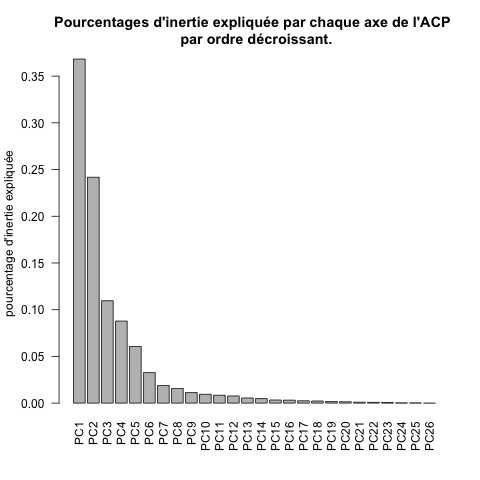
\includegraphics[width=0.5\textwidth]{imgs/acp.png}
        \caption{Pourcentages d'inertie expliquée}
        \label{fig_acp}
    \end{figure}

    Comme les 3 premiers axes factoriels représentent $72\%$ de la variance totale, nous analysons le nuage de points seulement avec les 3 premiers plans factoriels.
    Nous obtenons les plans factoriels des figures \ref{fig_acp_plan_1_2}, \ref{fig_acp_plan_1_3} et \ref{fig_acp_plan_2_3}. Nous avons associé à chaque plan son cercle des corrélations.
    
    \begin{figure}
        \centering
        \begin{subfigure}{.5\textwidth}
          \centering
          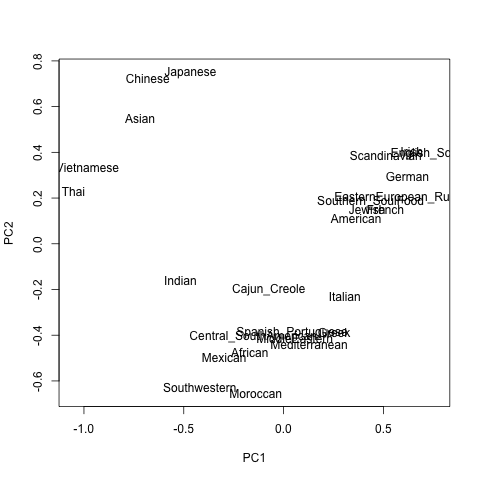
\includegraphics[width=.8\linewidth]{imgs/acp_plan_1_2.png}
          \caption{Plan 1,2}
          \label{fig:sub1}
        \end{subfigure}%
        \begin{subfigure}{.5\textwidth}
          \centering
          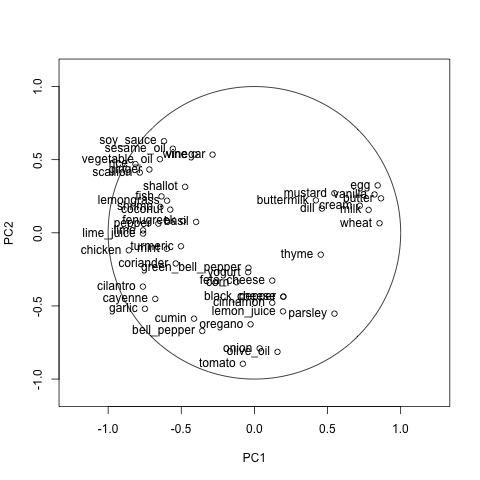
\includegraphics[width=.8\linewidth]{imgs/cercle_plan_1_2.png}
          \caption{Cercle des corrélations}
          \label{fig:sub2}
        \end{subfigure}
        \caption{Plan factoriel 1,2 avec son cercle associé}
        \label{fig_acp_plan_1_2}
    \end{figure}

    \begin{figure}
        \centering
        \begin{subfigure}{.5\textwidth}
          \centering
          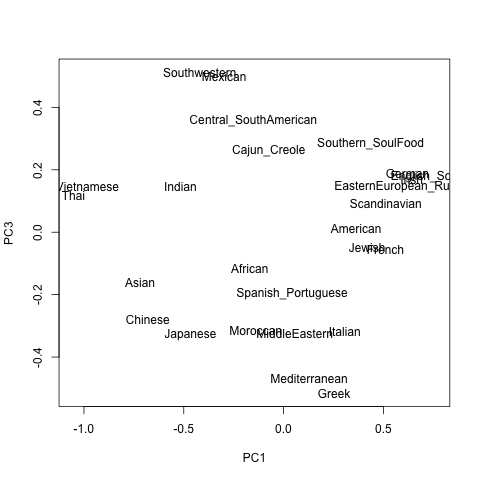
\includegraphics[width=.8\linewidth]{imgs/acp_plan_1_3.png}
          \caption{Plan 1,3}
          \label{fig:sub1}
        \end{subfigure}%
        \begin{subfigure}{.5\textwidth}
          \centering
          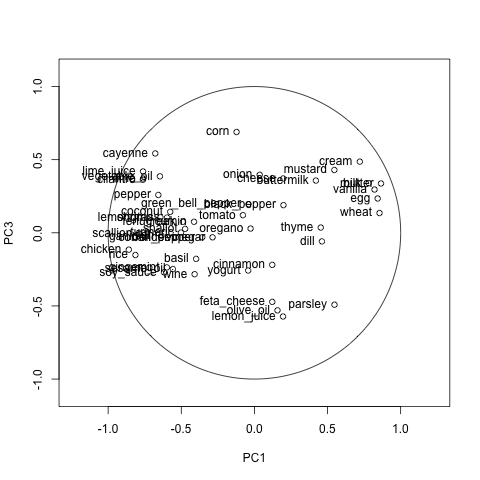
\includegraphics[width=.8\linewidth]{imgs/cercle_plan_1_3.png}
          \caption{Cercle des corrélations}
          \label{fig:sub2}
        \end{subfigure}
        \caption{Plan factoriel 1,3 avec son cercle associé}
        \label{fig_acp_plan_1_2}
    \end{figure}


    \begin{figure}
        \centering
        \begin{subfigure}{.5\textwidth}
          \centering
          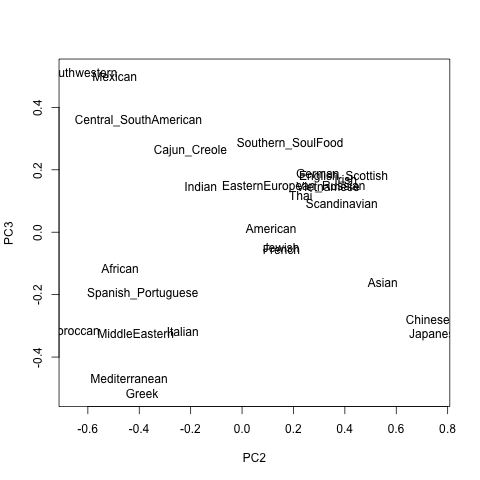
\includegraphics[width=.8\linewidth]{imgs/acp_plan_2_3.png}
          \caption{Plan 2,3}
          \label{fig:sub1}
        \end{subfigure}%
        \begin{subfigure}{.5\textwidth}
          \centering
          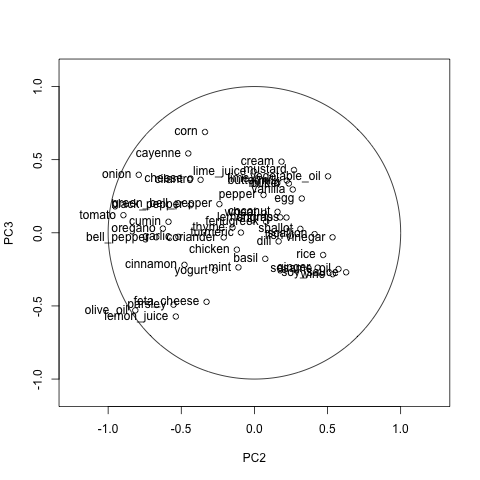
\includegraphics[width=.8\linewidth]{imgs/cercle_plan_2_3.png}
          \caption{Cercle des corrélations}
          \label{fig:sub2}
        \end{subfigure}
        \caption{Plan factoriel 2,3 avec son cercle associé}
        \label{fig_acp_plan_2_3}
    \end{figure}

    Dans le premier plan factoriel, nous observons que plusieurs groupes se forment.
    Les pays asiatiques se distinguent avec des ingrédients comme l'huile de sésame, l'huile de soja, le poisson, les échalottes...
    Un deuxième groupe se distingue: la cuisine occidentale avec des ingrédients comme le blé, les oeufs et le lait.
    Aussi, les pays consommant de la tomate et de l'huile d'olive sont exposés dans ce premier plan: Maroc, Mexique et Afrique.

    Dans le deuxième plan factoriel, la Grèce et la méditerranée sont liées par leur consommation de féta, d'huile d'olive et de jus de citron. 
    Ce plan permet aussi de voir la formation de deux sous groupes parmi les pays asiatiques.
    Le Vietnam et la Thaïlande consomment du poulet et du piment, ce qui est moins le cas de la Chine et du Japon.

    Enfin le troisième plan factoriel met en évidence des pays consommant du maïs comme le Mexique.

    \subsection*{Question 3}
    Nous obtenons le dendrogramme de la figure \ref{fig_CAH_dendrogramme}.
    
    \begin{figure}
        \centering
        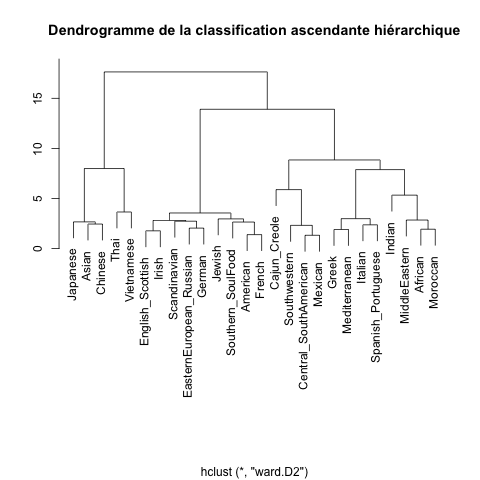
\includegraphics[width=0.5\textwidth]{imgs/CAH_dendrogramme.png}
        \caption{Dendrogramme de la classification ascendante hiérarchique}
        \label{fig_CAH_dendrogramme}
    \end{figure}

    Ce dendrogramme confirme plusieurs observations que nous avions déjà indiquées dans la deuxième question:
    \begin{itemize}
        \item les cuisines des pays asiatiques sont ensemble avec deux sous groupes: Japon-Chine, Thailande-Vietnam.
        \item les recettes de deux pays occidentaux, les Etats-Unis et la France, sont ensemble
        \item la cuisine méditerranée est regroupée avec les pays suivants: Grèce, Italie, Espagne, Portugal.
    \end{itemize}

    D'autres groupes que nous n'avions pas identifiés sont présents:
    \begin{itemize}
        \item les recettes des pays de l'europe de l'est avec l'Allemagne, la Russie et les pays de l'est.
        \item la cuisine des régions dans la partie inférieure au Texas: les Cadiens (présents au Texas et en Louisiane), Mexique, Amérique centrale, Amérique du sud.
        \item la cuisine d'Afrique et du Moyen-Orient (Afrique, Moyen-Orient et Maroc).
    \end{itemize}
    
    A un niveau plus macro nous avons 3 groupes:
    \begin{itemize}
        \item l'asie avec un indice de 7.5
        \item l'occident avec l'europe de l'est: un indice de 4 ce qui traduit une utilisation relativement homogène des ingrédients
        \item Amérique centrale et du sud, méditerranée, l'Inde, l'Afrique, avec un indice de 8 qui traduit une certaine hétérogénéité par rapport à l'occident par exemple
    \end{itemize}

    \subsection*{Question 4}

    Nous commençons par chercher quel serait un \"bon\" nombre de classes à choisir:
    \begin{figure}
        \centering
        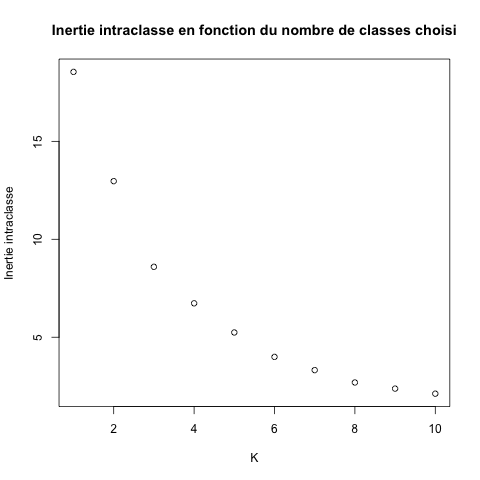
\includegraphics[width=0.5\textwidth]{imgs/K_means_choix_K.png}
        \caption{Inertie intraclasse en fonction du nombre de classes choisi}
        \label{fig_K_means_choix_K}
    \end{figure}

    En utilisant la règle du coude un nombre de classes est 3.
    Ce nombre est en adéquation avec la classification hiérarchique ascendante que nous avions obtenue dans la question précédente.
    En effet nous avions déjà identifié 3 groupes.

    Nous obtenons la classification suivante:
    \begin{center}
        \begin{tabular}{|l|l|l|}
            \hline
            1 & African, Cajun\_Creole, Central\_SouthAmerican, Greek, Indian, Italian, Mediterranean, Mexican, \\
            & MiddleEastern, Moroccan, Southwestern, Spanish\_Portuguese\\
            \hline
            2 & Asian, Chinese, Japanese, Thai, Vietnamese\\
            \hline
            3 & American, EasternEuropean\_Russian, English\_Scottish, French, German, Irish, Jewish,\\
            & Scandinavian, Southern\_SoulFood\\
            \hline
        \end{tabular}
    \end{center}
    Cette classification est identique aux trois groupes que nous avions identifié précedemment avec la CAH.

    \subsection*{Question 5}
    
    \subsection*{Question 6}

    \end{document}

